\documentclass[12pt,oneside]{book}
\usepackage[a4paper,top=2.5cm,bottom=2.5cm,left=3.5cm,right=2cm]{geometry}
\usepackage[utf8]{inputenc}
\usepackage[T1]{fontenc}
\usepackage{graphicx}
\usepackage{url}
\usepackage{amsmath}
\usepackage[slovak]{babel} % vypnite pre prace v anglictine
\linespread{1.25} % hodnota 1.25 by mala zodpovedat 1.5 riadkovaniu

% -------------------
% --- Definicia zakladnych pommov
% -------------------
\def\*{{\bf FIXME: }}
\def\mfyear{2016}
\def\mftitle{Vizualizácia evolučných histórií}
\def\mfthesistype{Bakalárska práca}
\def\mfauthor{Dávid Simeunovič}
\def\mfadvisor{doc. Mgr. Bronislava Brejová, PhD.}
\def\mfplacedate{Bratislava, \mfyear}
\def\odbor{2508 Informatka} %aj cislo odboru je povinne a je to podla katedry/odboru, na ktorom je autor
\def\program{ Informatika }
\def\stredisko{ Katedra Informatiky }

\def\mfrok{2016}
\def\mfnazov{Vizualizácia evolučných histórií}
\def\mftyp{Bakalárska práca}
\def\mfautor{Dávid Simeunovič}
\def\mfskolitel{doc. Mgr. Bronislava Brejová, PhD.}

%ak mate konzultanta, odkomentujte aj jeho meno na titulnom liste
\def\mfkonzultant{tit. Meno Priezvisko, tit. }  

\def\mfmiesto{Bratislava, \mfrok}

%aj cislo odboru je povinne a je podla studijneho odboru autora prace
\def\mfodbor{2508 Informatika} 
\def\program{ Informatika }
\def\mfpracovisko{ Katedra informatiky }

\begin{document}     

% -------------------
% --- Obalka ------
% -------------------
\thispagestyle{empty}

\begin{center}
\sc\large
Univerzita Komenského v Bratislave\\
Fakulta matematiky, fyziky a informatiky

\vfill

{\LARGE\mfnazov}\\
\mftyp
\end{center}

\vfill

{\sc\large 
\noindent \mfrok\\
\mfautor
}

\eject % EOP i
% --- koniec obalky ----

% -------------------
% --- Titulný list
% -------------------

\thispagestyle{empty}
\noindent

\begin{center}
\sc  
\large
Univerzita Komenského v Bratislave\\
Fakulta matematiky, fyziky a informatiky

\vfill

{\LARGE\mfnazov}\\
\mftyp
\end{center}

\vfill

\noindent
\begin{tabular}{ll}
Študijný program: & \program \\
Študijný odbor: & \mfodbor \\
Školiace pracovisko: & \mfpracovisko \\
Školiteľ: & \mfskolitel \\
% Konzultant: & \mfkonzultant \\
\end{tabular}

\vfill


\noindent \mfmiesto\\
\mfautor

\eject % EOP i


% --- Koniec titulnej strany


% -------------------
% --- Naskenovane Zadanie
% -------------------
% v tlačenej verzii s podpismi zainteresovaných osôb.
% v elektronickej verzii sa zverejňuje zadanie bez podpisov zainteresovaných osôb.

\newpage 
\thispagestyle{empty}
\hspace{-2cm}\includegraphics[width=1.1\textwidth]{images/zadanie}

% --- Koniec zadania

\frontmatter

% -------------------
%   Poďakovanie - nepovinné
% -------------------
\setcounter{page}{3}
\newpage 
~

\vfill
{\bf Poďakovanie:}


% --- Koniec poďakovania

% -------------------
%   Abstrankt - Slovensky
% -------------------
\newpage 
\section*{Abstrakt}

Táto práca sa venuje zobrazovaniu evolučných histórií. 
Výsledkom tejto práce je program \emph{EHDraw}, ktorý umožňuje vytvárať vizualizácie, 
meniť nastavenia použité pre tvorbu týchto vizualizácií a automaticky zredukovať počet génov, ktoré sa nachádzajú vo vizualizácii,
bez straty pre nás podstatnej informácie - aké mutácie sa odohrali v evolučnej histórii. 
Redukciu počtu génov transformujeme na Problém množinového pokrytia, jeho aproximáciu získame pomocou greedy algoritmu,
a jeho optimum pomocou Celočíselného lineárneho programovania. 
Rozdiely týchto dvoch prístupov porovnávame testami.
Výsledný program bude slúžiť na zobrazovanie a vizuálnu kontrolu výsledkov metód,
ktoré sa na základe dostupných DNA sekvencií snažia zrekonštruovať evolučnú históriu, ktorá by viedla k takýmto sekvenciám.  



\paragraph*{Kľúčové slová:} vizualizácia, evolučná história, výber génov, Problém množinového pokrytia,
greedy algoritmus, Celočíselné lineárne programovanie
% --- Koniec Abstrakt - Slovensky


% -------------------
% --- Abstrakt - Anglicky 
% -------------------
\newpage 
\section*{Abstract}
The subject of this work is visualisation of evolution histories.
The Result of this work is program \emph{EHDraw}, which allows creating visualisations and
changing their settings, It can also automatically reduce the number of genes contained in the visualisation,
without loss of relevant information for us, namely mutations which occurred in the evolution history.
Reduction of the number of genes is transformed to the Set Cover Problem, it's approximation is obtained by a greedy algorithm
and the optimal solution by Integer Linear Programming.
The differences of these two approaches are compared by tests.
Created program will allow visual control of the results of the methods, that based on the available DNA sequences
try to reconstruct the evolutionary history that would lead to such sequences.


\paragraph*{Keywords:}  visualisation, evolution history, gene selection, Set Cover Problem,
greedy algorithm, Integer Linear Programming

% --- Koniec Abstrakt - Anglicky

% -------------------
% --- Predhovor - v informatike sa zvacsa nepouziva
% -------------------
%\newpage 
%\thispagestyle{empty}
%
%\huge{Predhovor}
%\normalsize
%\newline
%Predhovor je všeobecná informácia o práci, obsahuje hlavnú charakteristiku práce 
%a okolnosti jej vzniku. Autor zdôvodní výber témy, stručne informuje o cieľoch 
%a význame práce, spomenie domáci a zahraničný kontext, komu je práca určená, 
%použité metódy, stav poznania; autor stručne charakterizuje svoj prístup a svoje 
%hľadisko. 
%
% --- Koniec Predhovor


% -------------------
% --- Obsah
% -------------------

\newpage 

\tableofcontents

% ---  Koniec Obsahu

% -------------------
% --- Zoznamy tabuliek, obrázkov
% -------------------

\newpage 

\listoffigures

% ---  Koniec Zoznamov

\mainmatter


\input uvod.tex 

\input biolog.tex

\input program.tex

\input setcover.tex

\input testovanie.tex

\input zaver.tex

% -------------------
% --- Bibliografia
% -------------------


\newpage	

\backmatter

\thispagestyle{empty}
\nocite{*}
\clearpage

\bibliographystyle{plain}
\bibliography{literatura} 

%Prípadne môžete napísať literatúru priamo tu
%\begin{thebibliography}{5}
 
%\bibitem{br1} MOLINA H. G. - ULLMAN J. D. - WIDOM J., 2002, Database Systems, Upper Saddle River : Prentice-Hall, 2002, 1119 s., Pearson International edition, 0-13-098043-9

%\bibitem{br2} MOLINA H. G. - ULLMAN J. D. - WIDOM J., 2000 , Databasse System implementation, New Jersey : Prentice-Hall, 2000, 653s., ???

%\bibitem{br3} ULLMAN J. D. - WIDOM J., 1997, A First Course in Database Systems, New Jersey : Prentice-Hall, 1997, 470s., 

%\bibitem{br4} PREFUSE, 2007, The Prefuse visualization toolkit,  [online] Dostupné na internete: <http://prefuse.org/>

%\bibitem{br5} PREFUSE Forum, Sourceforge - Prefuse Forum,  [online] Dostupné na internete: <http://sourceforge.net/projects/prefuse/>

%\end{thebibliography}

%---koniec Referencii

% -------------------
%--- Prilohy---
% -------------------

%Nepovinná časť prílohy obsahuje materiály, ktoré neboli zaradené priamo  do textu. Každá príloha sa začína na novej strane.
%Zoznam príloh je súčasťou obsahu.
%
%\addcontentsline{toc}{chapter}{Appendix A}
%\addcontentsline{prilohy.tex}{×}{×}
%\input prilohy.tex

%\addcontentsline{toc}{chapter}{Appendix B}
%\input AppendixB.tex

\end{document}






